\chapter{Evaluation}

To measure the effectiveness of dynamic windowing for multi-stream operators during the 
mapping of non-RDF heterogeneous data, we would need to measure the following 
metrics of our stream processing framework: \emph{latency}, \emph{throughput},
\emph{memory usage} and \emph{completeness}. \emph{Throughput}, in this 
paper, refers to the number of processed input records, per time unit.
\emph{Latency, throughput,} and \emph{memory usage} can be measured following the recent benchmark studies by 
Van Dongen and Van den Poel(2020)~\cite{evalution_of_spe}.
However, to evaluate 
for the \emph{completeness}
of the generated output, a reference output needs 
to be generated for comparison. Since a data stream is unbounded in nature, 
and cannot be processed completely to check for \emph{completeness}, a bounded 
dataset of relatively large volume will be used to measure \emph{completeness}.
To ensure consistency in the complexity of the multi-stream operator being used, 
we will apply the join operator in the windows --- a common operator used in 
data enrichment scenarios. 

The following sections will describe the methodology and the data used to evaluate the
different metrics. Setups required to reproduce the evaluation will also be elaborated 
in their respective sections. 


\section{Data}

Assessment of our dynamic windowing scheme for multi-stream operator will require 
the data to have some common attributes to enrich the data. Furthermore, to 
mirror a real-world scenario, we would also employ data gathered from IoT sensors. 
We will use the same data 
as is the case for the benchmark in the paper by Van Dongen and Van den Poel~\cite{evalution_of_spe}. 
The data is provided by NDW (Nationale Databank Wegverkeersgegevens) from the 
Netherlands~\footnote{NDW data site: \href{http://opendata.ndw.nu/}{http://opendata.ndw.nu/} }.
 It consists of measurements of the number of cars and their average speed. 
A subset of the complete sensor data will be replayed by a Kafka publisher into the two topics 
\emph{flow} and \emph{speed}, for the number of cars and the average speed respectively. 

\subsection{Data for completeness evaluation}
Completeness measure requires a dataset which could be mapped completely by a static 
mapping engine. 
Our \emph{complete} set of output triples will be generated according 
to the RML specification. Streaming data is usually 
ordered according to the event time, as defined in Chapter~\ref{chap:data_stream_processing} 
and the same entity could appear in the 
stream at a different timestamp. This can lead to duplicates in the generated output by 
the RMLMapper. Duplicates, in this context, are triples that semantically describe the 
same knowledge. Therefore, duplicates in the generated output by the reference optimal
mapping engine needs to be removed in the final \emph{complete} output dataset.

\section{Evaluation pipeline}

\begin{figure}[!htbp]
    \centering
    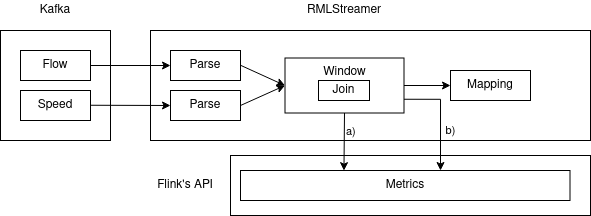
\includegraphics[width=\textwidth]{fig/evaluation_architecture.png}
    \caption{Evaluation flow based on~\cite{evalution_of_spe} with some changes to only 
    take metrics at the "Join" and the "Mapping" stage. a) \emph{throughput} of the generated output triple. 
    b) \emph{latency} of evaluating the join operator in windows.}
    \label{fig:evaluation_flow}
    
\end{figure}

Similar to the workflow process in~\cite{evalution_of_spe, benchmark_sce}, we set up
our evaluation pipeline as illustrated in Figure~\ref{fig:evaluation_flow}. Setting it 
up according to the illustrated pipeline, allows us to have fine control over the 
workload scenarios and limit the measurement of the metrics just to the windows. 




\section{Workload scenarios}
As stated in Chapter~\ref{chap:data_stream_processing}, data streams have characteristics 
which determine the performance of stream processing frameworks and its operators. Therefore, 
there is a need to evaluate our dynamic window implementation under different workload scenarios. 

\subsection{Workload for maximum throughput measurement}
This workload will attempt to measure the maximum throughput RMLStreamer can 
process with the different windows, before \emph{latency,} and \emph{memory utilization}
increase significantly~\cite{benchmark_dsdps}. We will increase the velocity of the input data gradually 
every 10 seconds until there is a significant latency of more than 10 seconds to produce
the next output triple or until the memory allocated to the instances get fully used up. 


\subsection{Workload for latency measurement}
As described in the paper by Van Dongen and Van den Poel~\cite{evalution_of_spe}, 
\emph{throughput} and \emph{latency} can affect each other if the workload is 
improperly configured. Therefore, measurement of the \emph{latency} caused only 
by the window implementations, requires the stream processing framework to not be 
stressed under significant \emph{throughput}. Thus, the Kafka broker will 
publish the records at a very low constant rate of around 200 messages per second. 

Since \emph{latency} is also measured with a time unit, the timestamp of the 
records are important for \emph{latency} measurement. Due to the replay of the dataset 
by the Kafka broker, it is imperative to use the local timestamp of the same Kafka broker
attached to the input and output records for \emph{latency} 
measurement\cite{latency_measurement_kafka}.

\subsection{Workload for failure restart}
Evaluating the performance of dynamic windows to handle a restart in case of failure  
will stress test the implementation to handle the initial burst of data.
This is to emulate the scenario where RMLStreamer has to catch up with processing 
the records after a node failure. The Kafka 
broker will be started first to buffer the data stream for 5 minutes at a constant rate 
of around 1000 messages per second. Afterwards, RMLStreamer will be started to begin 
processing the records to catch up with the data stream. Once the RMLStreamer is started, 
Kafka broker will slow down the publishing of records to allow the RMLStreamer to catch
up.

\subsection{Workload for completeness}
The implementation of the dynamic window should also ensure that the generated 
output is as \emph{complete} as possible. The bounded dataset will be processed fully by 
a reference optimal mapping engine. The generated RDF graph by the reference 
optimal engine will be \emph{complete}. It will be used to compare with the result 
generated by the RMLStreamer for each window being evaluated. 

Depending on the type of window being used, \emph{completeness} of the output will be
affected by the window size. If the window size is not sufficiently large enough to handle 
the input velocity, the next incoming record will be processed in the new window instead of 
the old window where it is more relevant to the other records in the old window. Thus, 
we will vary the stream rate to measure the \emph{completeness} of the results generated 
with the use of different windows.

\subsection{Workload with periodic burst}
Fluctuation in the streaming sources are normal with unstable network connections. 
The windowing operator must therefore be able to cope with sudden changes in the 
fluctuation of the velocity of the data stream. This workload attempts to emulate 
the scenario where multiple IoT devices sends data in bursts with a periodic 
time interval. The workload will have a constant low stream rate with occasional 
bursts of data every few seconds. 


\section{Environment}

RMLStreamer will be evaluated in a virtual environment provided imec IDLabt from Ghent 
University called Virtual Wall\footnote{Virtual Wall: \href{https://doc.ilabt.imec.be/ilabt/virtualwall/index.html}{https://doc.ilabt.imec.be/ilabt/virtualwall/index.html}}.
Virtual Wall provides us with machines to run our tests remotely with consistent 
hardware specifications. It also provides the developers with the ability to induce 
artificial network impairment such as delay, packet loss, and bandwidth limitation. Such 
flexibility in the configuration allow us to devise a scenario as close to a real-world use case. 

For this work, we will be making use of it to set up the testing 
environment and mimic it as closely as possible to a real-world scenario. 
To prevent the publishing of data from taking up the resources used for evaluating the 
window operators, a Kafka broker will be run on a separate node. RMLStreamer will then be 
executed on a standalone node. Only a single Kafka broker will be used throughout the experiment, 
to ensure that the \emph{latency} measurement all comes from the same wall clock of the machine. 
Different Kafka brokers could be used in the experiment and then synchronized again 
with Network Time Protocol (NTP). However, the latency will still have a minimum
error of 35 ms~\cite{ntp_latency}, which is not suitable to measure the sub 10ms latencies in 
real-time applications. Therefore, we opted to use only a single Kafka broker to publish
our data stream for evaluation.





